\documentclass{amsart}
\usepackage{amsmath, amsthm, amssymb}
\usepackage{tikz}
\usetikzlibrary{arrows.meta}

\begin{document}

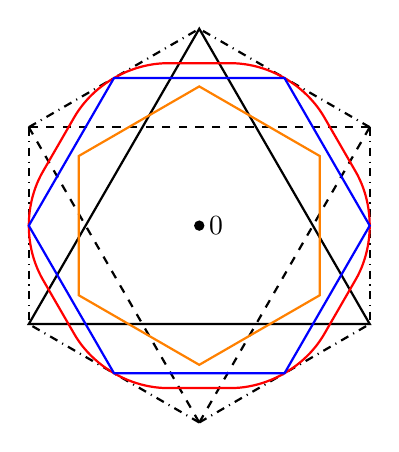
\begin{tikzpicture}[scale=1.25]
\def\p{3};


\draw[thick] ({-sqrt(3)},-1) -- ({sqrt(3)},-1) -- (0,2) -- cycle;


\draw[dashed,thick] ({sqrt(3)},1) -- ({-sqrt(3)},1);
\draw[dashed,thick] ({-sqrt(3)},1) -- (0,-2);
\draw[dashed,thick] (0,-2) -- ({sqrt(3)},1);


\draw[dashdotted,thick] (0,-2) -- ({-sqrt(3)},-1);
\draw[dashdotted,thick] (0,-2) -- ({sqrt(3)},-1);
\draw[dashdotted,thick] ({sqrt(3)},1) -- ({sqrt(3)},-1);
\draw[dashdotted,thick] ({sqrt(3)},1) -- (0,2);
\draw[dashdotted,thick] ({-sqrt(3)},1) -- (0,2);
\draw[dashdotted,thick] ({-sqrt(3)},1) -- ({-sqrt(3)},-1);


\draw[red,thick,variable=\t,domain={1/(2^(\p-1)+1)}:{2^(\p-1)/(2^(\p-1)+1)}] 
		plot	(	{-sqrt(3)*(1-\t) / (2^(1/\p) * (\t^(\p/(\p-1))+(1-\t)^(\p/(\p-1)))^((\p-1)/\p))},
				{(-(1-\t) -2*\t) / (2^(1/\p) * (\t^(\p/(\p-1))+(1-\t)^(\p/(\p-1)))^((\p-1)/\p))}	)
	--	plot	(	{sqrt(3)*\t / (2^(1/\p) * (\t^(\p/(\p-1))+(1-\t)^(\p/(\p-1)))^((\p-1)/\p))},
				{(-2*(1-\t) - \t) / (2^(1/\p) * (\t^(\p/(\p-1))+(1-\t)^(\p/(\p-1)))^((\p-1)/\p))}	)
	--	plot	(	{sqrt(3) / (2^(1/\p) * (\t^(\p/(\p-1))+(1-\t)^(\p/(\p-1)))^((\p-1)/\p))},
				{(2*\t -1) / (2^(1/\p) * (\t^(\p/(\p-1))+(1-\t)^(\p/(\p-1)))^((\p-1)/\p))}	)
	--	plot	(	{sqrt(3)*(1-\t) / (2^(1/\p) * (\t^(\p/(\p-1))+(1-\t)^(\p/(\p-1)))^((\p-1)/\p))},
				{((1-\t) + 2*\t) / (2^(1/\p) * (\t^(\p/(\p-1))+(1-\t)^(\p/(\p-1)))^((\p-1)/\p))}	)
	--	plot	(	{-sqrt(3)*\t / (2^(1/\p) * (\t^(\p/(\p-1))+(1-\t)^(\p/(\p-1)))^((\p-1)/\p))},
				{(2*(1-\t) + \t)) / (2^(1/\p) * (\t^(\p/(\p-1))+(1-\t)^(\p/(\p-1)))^((\p-1)/\p))}	)
	--	plot	(	{-sqrt(3) / (2^(1/\p) * (\t^(\p/(\p-1))+(1-\t)^(\p/(\p-1)))^((\p-1)/\p))},
				{(-\t + (1-\t)) / (2^(1/\p) * (\t^(\p/(\p-1))+(1-\t)^(\p/(\p-1)))^((\p-1)/\p))}	)
	--		cycle;


\draw[blue,thick] ({-sqrt(3)},0) -- ({-sqrt(3)/2},-1.5) -- ({sqrt(3)/2},-1.5) -- ({sqrt(3)},0) -- ({sqrt(3)/2},1.5) -- ({-sqrt(3)/2},1.5) -- cycle;


\draw[orange,thick] ({sqrt(3/2)},{sqrt(1/2)}) -- (0,{sqrt(2)}) -- ({-sqrt(3/2)},{sqrt(1/2)})
			-- ({-sqrt(3/2)},{-sqrt(1/2)}) -- (0,{-sqrt(2)}) -- ({sqrt(3/2)},{-sqrt(1/2)}) -- cycle;


\fill (0,0) circle [radius=1.5pt] node[anchor=west] {0};
\end{tikzpicture}

\end{document}